\documentclass{exam}
\usepackage{main}

\title{Evaluation de Cours}
\date{7 Mars 2024}
\author{Maths Spécifiques}

\begin{document}
\maketitle
\thispagestyle{empty}
\section*{Version 1}
\begin{questions}
\question Soit $\function{f}{\R}{\R}{x}{-x + 3}$.
\begin{parts}
\part Identifier le coefficient directeur et l'ordonnée à l'origine de $f$.
\part La courbe $\mathcal{C}$ représentée ci-après est-elle la courbe représentative de $f$ ? Justifier votre réponse.
\vspace*{1cm}
\begin{center}
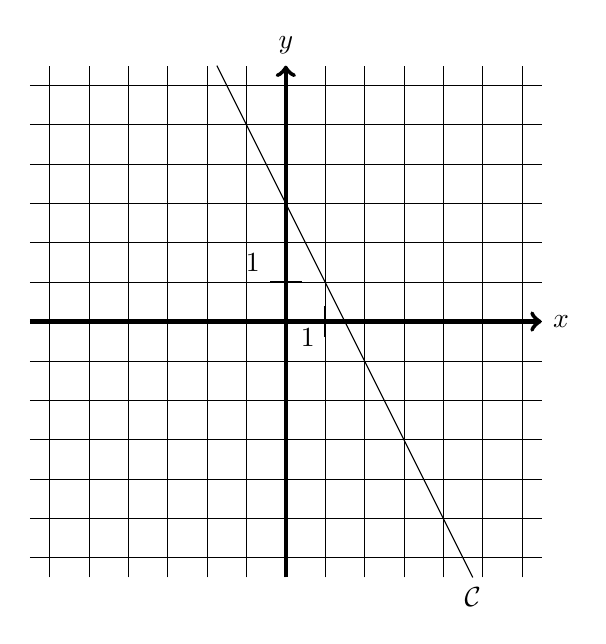
\begin{tikzpicture}
\draw[line width = 0.01cm] (-3.25,-3.25) grid[step=0.5] (3.25,3.25);
\draw[ultra thick,->] (-3.25,0) -- (3.25,0) node[right] {$x$};
\draw[ultra thick,->] (0,-3.25) -- (0,3.25) node[above] {$y$};
\draw[thick] (0.5,0.2) -- (0.5,-0.2) node[left] {$1$};
\draw[thick] (0.2,0.5) -- (-0.2,0.5) node[above left] {$1$};
\draw (-0.875,3.25) -- (2.375,-3.25) node[below] {$\mathcal{C}$};
\end{tikzpicture}
\end{center}
\end{parts}
\end{questions}

\newpage

\maketitle
\thispagestyle{empty}
\section*{Version 2}
\begin{questions}
\question Soit $\function{f}{\R}{\R}{x}{-2x + 3}$.
\begin{parts}
\part Identifier le coefficient directeur et l'ordonnée à l'origine de $f$.
\part La courbe $\mathcal{C}$ représentée ci-après est-elle la courbe représentative de $f$ ? Justifier votre réponse.
\vspace*{1cm}
\begin{center}
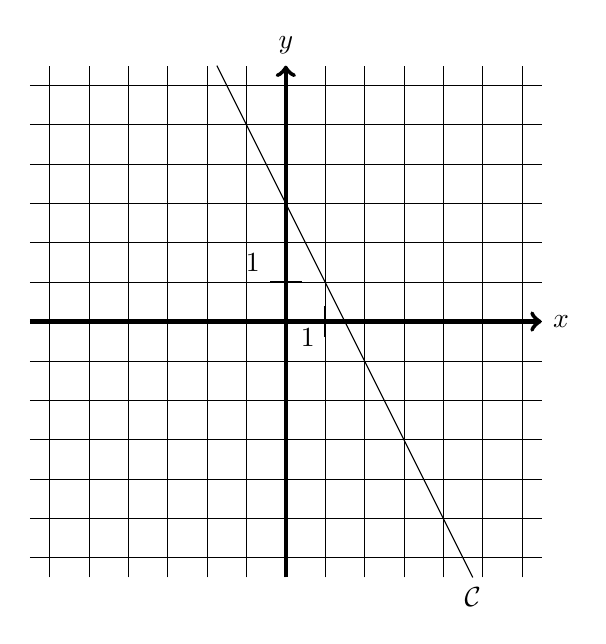
\begin{tikzpicture}
\draw[line width = 0.01cm] (-3.25,-3.25) grid[step=0.5] (3.25,3.25);
\draw[ultra thick,->] (-3.25,0) -- (3.25,0) node[right] {$x$};
\draw[ultra thick,->] (0,-3.25) -- (0,3.25) node[above] {$y$};
\draw[thick] (0.5,0.2) -- (0.5,-0.2) node[left] {$1$};
\draw[thick] (0.2,0.5) -- (-0.2,0.5) node[above left] {$1$};
\draw (-0.875,3.25) -- (2.375,-3.25) node[below] {$\mathcal{C}$};
\end{tikzpicture}
\end{center}
\end{parts}
\end{questions}
\end{document}